\documentclass[UTF8,a4paper,12pt]{ctexart}



%----------各种package----------%
\usepackage{amsmath, amsthm, amssymb, bm, graphicx, mathrsfs}
%超链接跳转,不显示边框但换颜色
\usepackage[colorlinks, linkcolor=red, urlcolor=blue]{hyperref}
%%-----设置section样式-----%%
\CTEXsetup[format={\Large\bfseries}]{section}                        %设置章标题字号为large,居左
\CTEXsetup[format={\large\bfseries}]{subsection}     
\CTEXsetup[format={\large\bfseries}]{subsubsection}     
\CTEXsetup[name={,、}]{section}  %标题设置为一、二、三、...
\CTEXsetup[number={\chinese{section}}]{section}                      %section形式改为一,二,三,..
 
\CTEXsetup[name={(,)}]{subsection}                                 
\CTEXsetup[number={\chinese{subsection}}]{subsection}                %subsection形式改为(一,二,三,...)
                            
\CTEXsetup[number=\arabic{subsubsection}]{subsubsection}    %subsubsection形式改为1,2,3,..
%%-----设置section样式-END-----%%
\usepackage{fancyhdr} %页眉
\usepackage{appendix} %附录
%页边距等
\usepackage[left=3.17cm, right=3.17cm, top=2.74cm, bottom=2.74cm]{geometry}

\usepackage{subfigure} %不言自明

\usepackage[linesnumbered,ruled,vlined]{algorithm2e} %伪代码

%----------代码---------
\usepackage[dvipsnames]{xcolor}
\usepackage{xcolor} 
\usepackage{listings} 
\lstset{ 
breaklines,%自动换行
basicstyle=\small,
escapeinside=``,
keywordstyle=\color{ blue!70} \bfseries,
commentstyle=\color{red!50!green!50!blue!50},% 
stringstyle=\ttfamily,% 
extendedchars=false,% 
linewidth=\textwidth,% 
numbers=left,% 
numberstyle=\tiny \color{blue!50},% 
frame=trbl% 
rulesepcolor= \color{ red!20!green!20!blue!20} 
}
%-----------------------
%----------各种package-END----------%








\linespread{1.5}
\newtheorem{theorem}{定理}[section]
\newtheorem{definition}[theorem]{定义}
\newtheorem{lemma}[theorem]{引理}
\newtheorem{corollary}[theorem]{推论}
\newtheorem{example}[theorem]{例}
\newtheorem{proposition}[theorem]{命题}
\pagestyle{fancy}%清除原页眉页脚样式
\fancyhf{} 



\begin{document}
%-------!!!一定记得修改的地方!!!-------%
\title{{\Huge{\textbf{实验报告常规模板}}}\\——Znamya自用模板}
\author{Znamya\\2213218@mail.nankai.edu.cn}
\date{\today}
%R:页面右边%L:页面左边%C:页面中间

\fancyhead[L]{\leftmark}%\leftmark:表示“一级标题”

\fancyhead[C]{实验报告}%\rightmark:表示“二级标题”

\fancyhead[R]{\thepage}%\thepage:表示“页码”

%-------!!!一定记得修改的地方!!!-End-------%
% \thispagestyle{empty} %放在这里没用!

\begin{figure}[t]
\vspace{-8cm}
\begin{center}
    
\includegraphics[width=0.6\textwidth]{figs/NKU.png}
\end{center}
\maketitle
\end{figure}
\thispagestyle{empty} %去除第一页的页码

\clearpage






% \maketitle

\pagenumbering{roman}
% \setcounter{page}{1}

% \begin{center}
%     \Huge\textbf{前言}
% \end{center}~\

% 这是笔记的前言部分. 
% ~\\
% \begin{flushright}
%     \begin{tabular}{c}
%         Znamya\\
%         \today
%     \end{tabular}
% \end{flushright}

% \newpage
\pagenumbering{Roman}
\setcounter{page}{1}
\tableofcontents
\newpage
\setcounter{page}{1}
\pagenumbering{arabic}

% \chapter{章节标题}

\begin{abstract}
    本文为Znamya的自用实验报告模板(虽然本科需要写报告的日子也不多了?),虽说是实验报告模板,用于其它场合也是完全可以的。
\end{abstract}

\section{图片}
\subsection{双图}

\begin{figure*}[h!]
	% \hspace{-1.5em}
    \centering
	\begin{tabular}{cccc}

		\subfigure[子图1]{
			\begin{minipage}[t]{0.5\textwidth}
				\centering
				\label{a}
				%% \hspace{-0.5em}
				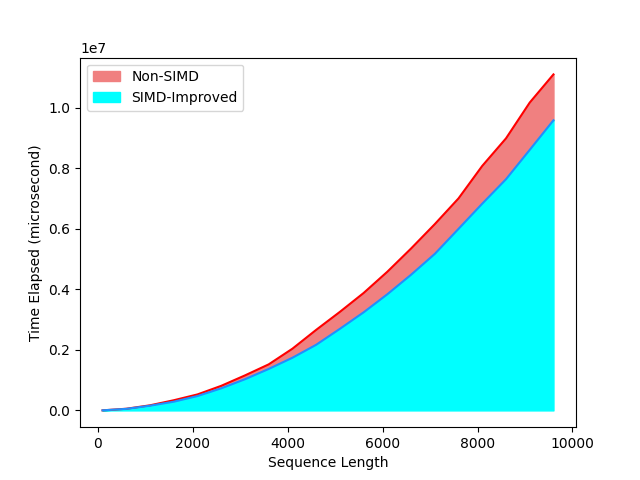
\includegraphics[width=2.8in]{figs/example-plot.png}
				%\vspace{0.5em}
		\end{minipage}}

        % \hspace{-0.5cm}

        \subfigure[子图2]{
			\begin{minipage}[t]{0.5\textwidth}
				\centering
				\label{a}
				%% \hspace{-0.5em}
				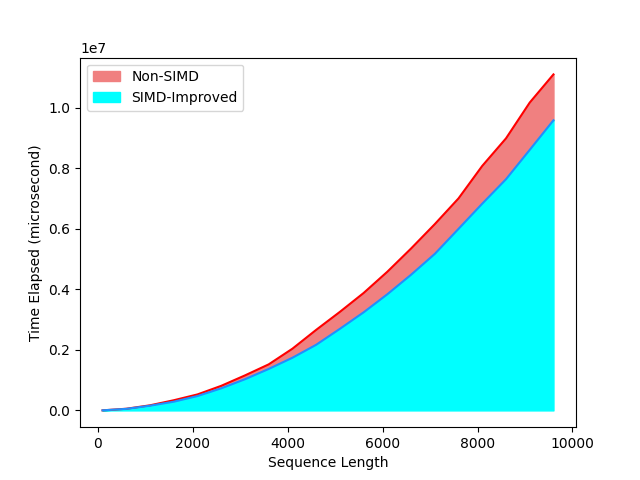
\includegraphics[width=2.8in]{figs/example-plot.png}
				%\vspace{0.5em}
		\end{minipage}}

        % \hspace{-0.5cm}

    	\end{tabular}
	% \vspace{-0.8em}
	\caption{两个子图并排}
	\label{fig:two-subfigs}
	\vspace{-1.3em}
\end{figure*}


\subsection{三图}
\begin{figure*}[h!]
	% \hspace{-1.5em}
    \centering
	\begin{tabular}{cccc}

		\subfigure[子图1]{
			\begin{minipage}[t]{0.3\textwidth}
				\centering
				\label{a}
				%% \hspace{-0.5em}
				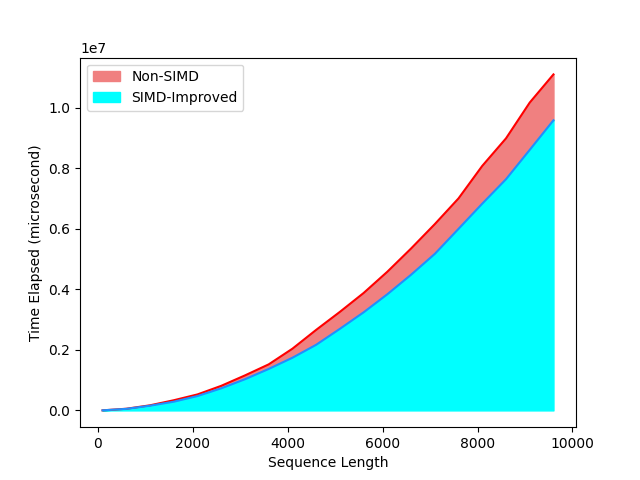
\includegraphics[width=1.8in]{figs/example-plot.png}
				%\vspace{0.5em}
		\end{minipage}}

        % \hspace{-0.5cm}

        \subfigure[子图2]{
			\begin{minipage}[t]{0.3\textwidth}
				\centering
				\label{a}
				%% \hspace{-0.5em}
				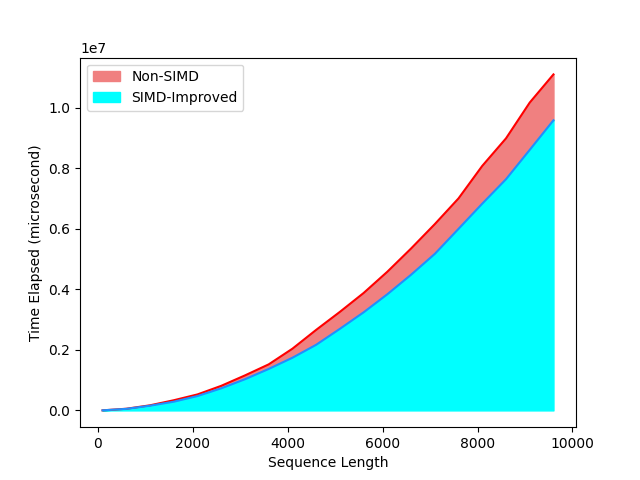
\includegraphics[width=1.8in]{figs/example-plot.png}
				%\vspace{0.5em}
		\end{minipage}}

        % \hspace{-0.5cm}

        \subfigure[子图3]{
			\begin{minipage}[t]{0.3\textwidth}
				\centering
				\label{a}
				%% \hspace{-0.5em}
				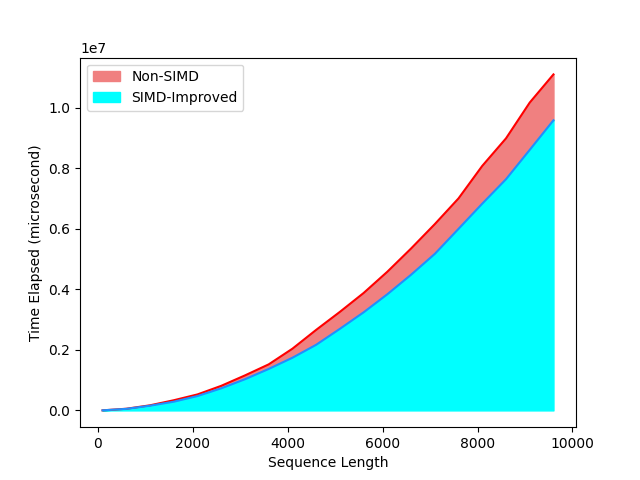
\includegraphics[width=1.8in]{figs/example-plot.png}
				%\vspace{0.5em}
		\end{minipage}}

    	\end{tabular}
	% \vspace{-0.8em}
	\caption{三个子图并排}
	\label{fig:three-subfigs}
	\vspace{-1.3em}
\end{figure*}


\subsection{多行图片}
本质上就是加了个换行。



\begin{figure*}[h!]
	% \hspace{-1.5em}
    \centering
	\begin{tabular}{cccc}

		\subfigure[子图1]{
			\begin{minipage}[t]{0.3\textwidth}
				\centering
				\label{a}
				%% \hspace{-0.5em}
				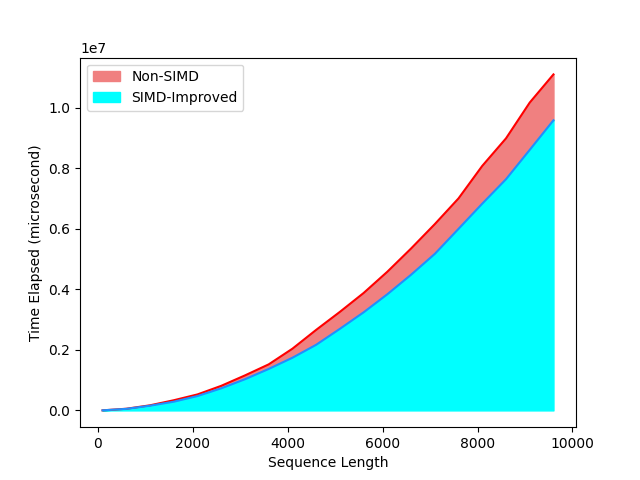
\includegraphics[width=1.8in]{figs/example-plot.png}
				%\vspace{0.5em}
		\end{minipage}}

        % \hspace{-0.5cm}

        \subfigure[子图2]{
			\begin{minipage}[t]{0.3\textwidth}
				\centering
				\label{a}
				%% \hspace{-0.5em}
				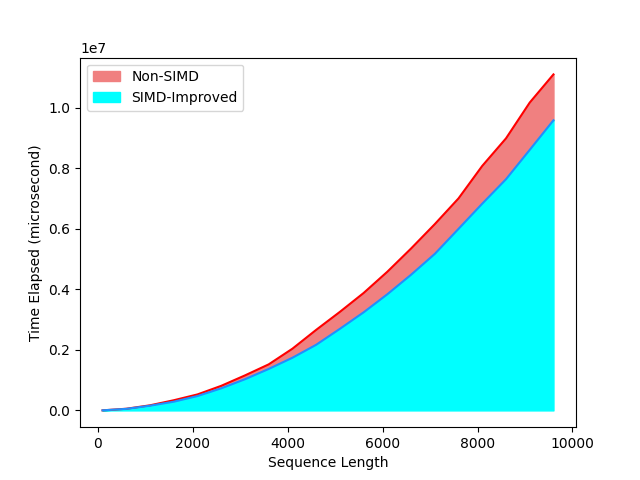
\includegraphics[width=1.8in]{figs/example-plot.png}
				%\vspace{0.5em}
		\end{minipage}}

        % \hspace{-0.5cm}

        \subfigure[子图3]{
			\begin{minipage}[t]{0.3\textwidth}
				\centering
				\label{a}
				%% \hspace{-0.5em}
				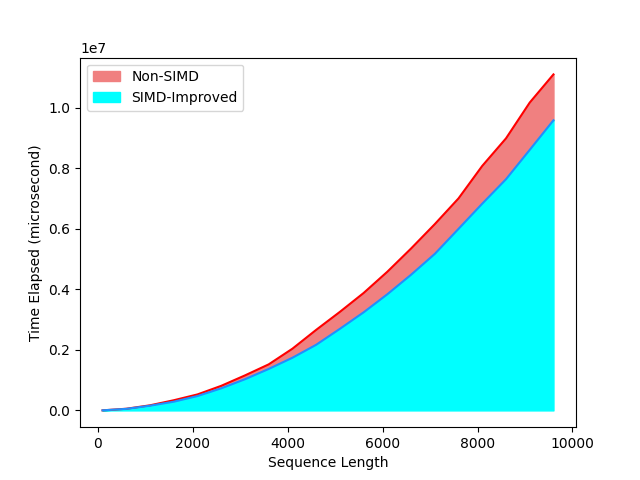
\includegraphics[width=1.8in]{figs/example-plot.png}
				%\vspace{0.5em}
		\end{minipage}}

        \\
        \

        \subfigure[子图1]{
			\begin{minipage}[t]{0.3\textwidth}
				\centering
				\label{a}
				%% \hspace{-0.5em}
				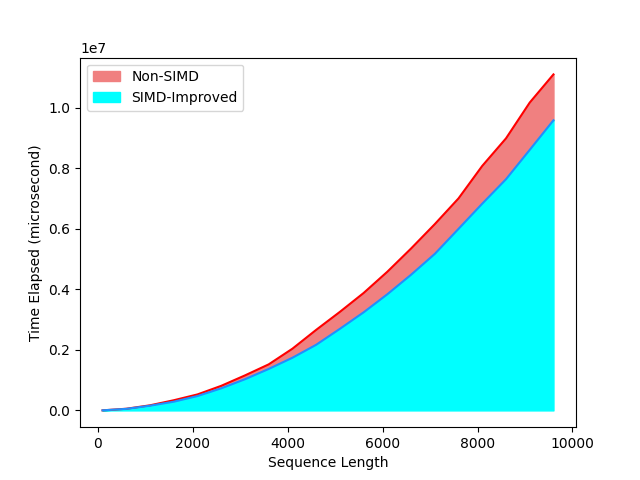
\includegraphics[width=1.8in]{figs/example-plot.png}
				%\vspace{0.5em}
		\end{minipage}}

        % \hspace{-0.5cm}

        \subfigure[子图2]{
			\begin{minipage}[t]{0.3\textwidth}
				\centering
				\label{a}
				%% \hspace{-0.5em}
				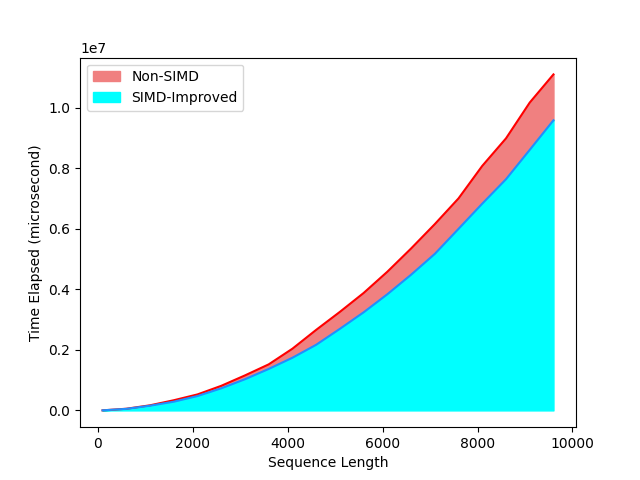
\includegraphics[width=1.8in]{figs/example-plot.png}
				%\vspace{0.5em}
		\end{minipage}}

        % \hspace{-0.5cm}

        \subfigure[子图3]{
			\begin{minipage}[t]{0.3\textwidth}
				\centering
				\label{a}
				%% \hspace{-0.5em}
				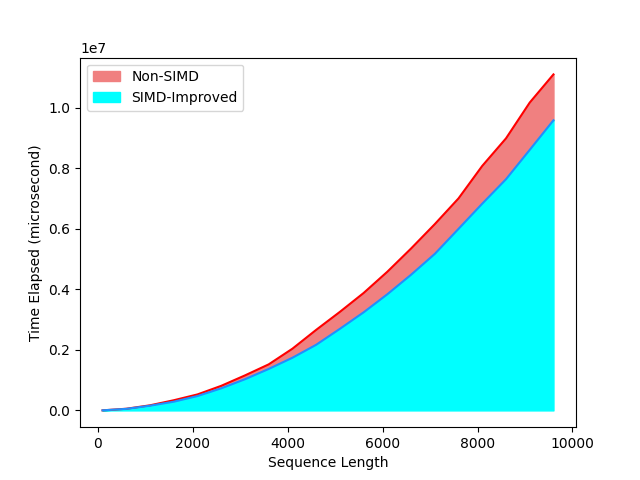
\includegraphics[width=1.8in]{figs/example-plot.png}
				%\vspace{0.5em}
		\end{minipage}}
    	\end{tabular}
	% \vspace{-0.8em}
	\caption{两行图片并排}
	\label{fig:two-row-subfigs}
	\vspace{-1.3em}
\end{figure*}

\section{代码块}
更多listing参数请上网搜索。
\begin{lstlisting}[   % 进行参数设置
    language=Python, % 设置语言
    basicstyle=\ttfamily\footnotesize, % 设置字体族
    breaklines=true, % 自动换行
    keywordstyle=\bfseries\color{NavyBlue}, % 设置关键字为粗体,颜色为 NavyBlue
    morekeywords={}, % 设置更多的关键字,用逗号分隔
    emph={self}, % 指定强调词,如果有多个,用逗号隔开
    emphstyle=\bfseries\color{Rhodamine}, % 强调词样式设置
    commentstyle=\itshape\color{black!50!white}, % 设置注释样式,斜体,浅灰色
    stringstyle=\bfseries\color{PineGreen!90!black}, % 设置字符串样式
    title=CNN模型的基本架构
]  
def __init__(self, vocab_size, embedding_dim, n_filters,
        filter_sizes, output_dim, dropout_rate, pad_index,):
    super().__init__()
    # 嵌入层,用于单词的语义感知
    self.embedding = nn.Embedding(embedding_dim=embedding_dim, num_embeddings=vocab_size)
    # 多个一维卷积层,注意其中需要对filter列表进行遍历
    self.convs = nn.ModuleList(
        [nn.Conv1d(in_channels=embedding_dim, out_channels=n_filters, kernel_size=fs)
        for fs in filter_sizes])
    # 全连接层
    self.fc = nn.Linear(in_features=len(filter_sizes)*n_filters, out_features=output_dim)
    # 在卷积和全连接之间引入dropout避免过拟合
    self.dropout = nn.Dropout(dropout_rate)
\end{lstlisting} 


\section{伪代码}
\begin{algorithm}[htbp]
	\caption{伪代码示例}\label{alg:example}
	% \DontPrintSemicolon
    \SetAlgoLined %显示end
	\SetKwInOut{Input}{输入}
	\SetKwInOut{Output}{输出}
	\Input{随便驶入一点什么}
	\Output{随便输出一点什么}
	\BlankLine
    $a=123456789$\\
	$b \leftarrow abcdef$\tcp{随便什么注释}
    \For{condition}{
		only if\;
		\If{condition}{
			1\;
		}
	}
	\While{not at end of this document}{
		if and else\;
		\eIf{condition}{
			1\;
		}{
			2\;
		}
	}
	\ForEach{condition}{
		\If{condition}{
			1\;
		}
	}
\end{algorithm}


\section{常用的正文格式}
这是笔记的正文部分. 本模板参考了知乎\cite{自用模板}和CSDN上的一些文章,部分致谢参见repository根目录\footnote{本latex文件是github一个仓库中的内容,参见\url{https://github.com/FeliceRivarez/Rivarez-LatexTemplate}}的readme.md。文中引用可以使用ref指令来进行,例如:图\ref{fig:three-subfigs},伪代码\ref{alg:example}。
\subsection{bibtex的使用}
直接把引文的bib格式文本放到LabReport.bib即可。对于链接等不便归类为论文或者书籍的,可以直接用Misc,用法参见LabReport.bib。

\subsubsection{bibtex注意事项}
注意格式规范即可,一般实验无所谓了。




%参考文献
\bibliographystyle{plain}
\bibliography{LabReport}



%附录
\begin{appendices}
\CTEXsetup[number=\Alph{section}]{section} 
\section{附录:测试1}
附录内容
\section{附录:测试2}
...
\end{appendices}
\end{document}